\begin{scanpage}{0123}{106}
\begin{center}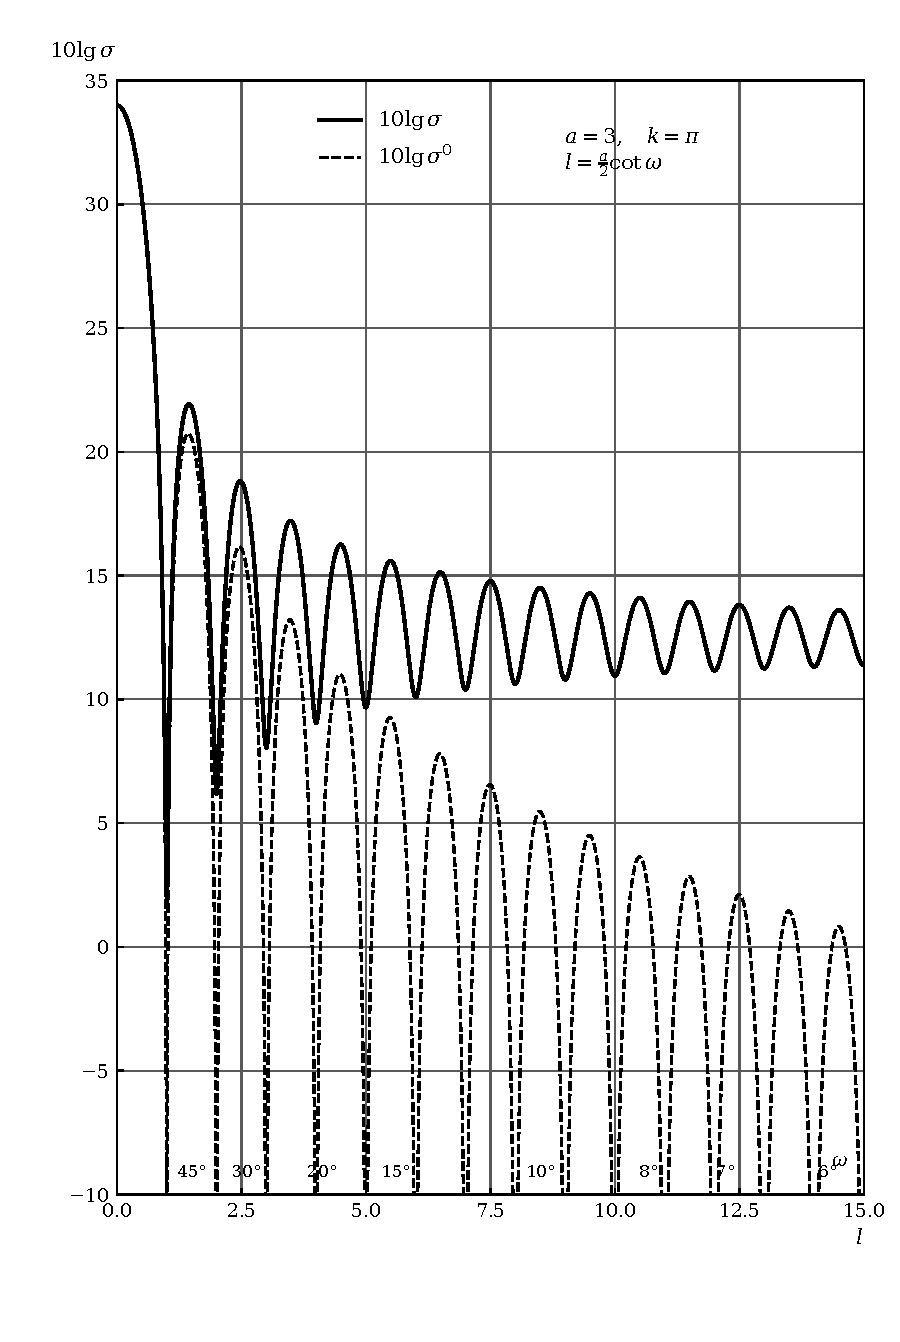
\includegraphics[width=.65\linewidth]{images/recreated/b-0123-fig38.pdf}

\begin{minipage}{.70\linewidth}Figure 38. The effective scattering area of a finite paraboloid as a function of its length with a constant radius of the base.\end{minipage}\end{center}
As in the case of a cone, the shape of the shadowed part turns out to have a substantial influence on the reflected signal. For example, for a paraboloid with the parameters $ka=2\pi$, $kl=10\pi$, $\operatorname{tg}\omega=0.1$ $(k=\pi)$, the reflected signal increases by 44 dB with an increase of $\Omega$ $(\omega<\Omega<\pi-\omega)$ (Figure 39).
\end{scanpage}
